\section{Background}
\subsection{Bayesian Statistics}
This paper does not aim to serve as a guide to Bayesian statistics or an
explicit introduction to the theory. Nonetheless, background knowledge is
necessary to understand the theory and assumptions motivated throughout the
paper.

In Bayesian statistics, the foundational interpretation of probability differs
from traditional frequentist statistics. In the more familiar frequentist approach,
probability is defined as the long-run frequency of an event occurring, the
intuition of which can be built with the example of a coin flip. The
probability of a coin landing on heads is assumed to be a fixed but unknown
quantity, and when a coin is flipped 100 times, and 70 of those flips result in
heads, the probability of heads is defined as 0.7.

In contrast, Bayesian statistics defines probability as a measure of belief and
model parameters - like the true fairness of a coin - are assumed to be random
variables. Our belief about the probability of heads is first explicitly
defined and then updated based on observed data. 
This prior belief could be based on a fair coin assumption (50-50 chance) or any other
prior knowledge. Then, as data is gathered from coin flips, this belief is
adjusted.
For instance, if a coin is flipped 100 times and heads appear 70 times, this
information is considered to revise the initial belief about the coin's
fairness. The updating process leans on the side of the observed data. In other
words, the more often heads appear in the flips, the more the belief tilts
towards thinking the coin is biased towards heads.
This updated belief incorporates the observed data and the initial belief,
offering a revised understanding of the coin's behaviour. The Bayesian approach,
therefore, provides a systematic way of refining beliefs in light of new
evidence, resulting in a flexible framework for making predictions - or
inferences - about future events.

Take two events, $A$ and $B$, where the probability of an event is given by
$P(Event)$; the probability of event $A$ given event $B$ is given by $P(A|B)$.
Because the probability $P$ is defined as a measure of belief, the probability
of an event $A$, given by $P(A)$, is precisely the belief in the occurrence of
event $A$, instead of being the proportion of times event $A$ would occur if
the experiment were hypothetically repeated an infinite number of times - this
frequentist perspective is fundamentally tied to repeatable random events. This
means that, in Bayesian statistics, probability can be assigned to any
statement whatsoever, even when no random process is involved. So the
probability of $A$ given $B$, $P(A|B)$, models belief in the occurrence of event
$A$ given that event $B$ has occured and is the underlying essence of Bayesian
thinking.
\subsubsection{Bayes' Theorem}
The framework for updating beliefs in Bayesian statistics is Bayes' theorem,
derived from the definition of conditional probability. Bayes' theorem
describes the probability of an event based on prior knowledge of conditions
that might be related to the event and observed evidence. For events $A$ and
$B$, the general form of Bayes' theorem is given by:
\begin{equation}
  P(A|B) = \frac{P(B|A)P(A)}{P(B)}
\end{equation}
Applications of the Bayesian framework are vast; the belief in any hypothesis
can be logically updated when new evidence is encountered.
\begin{equation}
  P(\text{Hypothesis}|\text{Evidence}) = \frac{P(\text{Evidence}|\text{Hypothesis})P(\text{Hypothesis})}{P(\text{Evidence})}
\end{equation}
In the context of Bayesian modelling, the focus is on updating our beliefs
about the parameters of a model, given some observed data.
\begin{equation}
  \label{eq:bayes_theorem}
  P(\text{Parameters}|\text{Data}) = \frac{P(\text{Data}|\text{Parameters})P(\text{Parameters})}{P(\text{Data})}
\end{equation}
Equation \ref{eq:bayes_theorem} is the Holy Grail of Bayesian modelling, and
its components make up the most important and frequently used terms in Bayesian
statistics. Table \ref{tab:bayes_theorem} labels these components; the
posterior is, by the definition of probability in Bayesian
statistics, the belief in the parameters given the observed data - all
parametric modelling, Bayesian or not, is asking this question to a degree.
In this context, Bayes' theorem elegantly demonstrates how our initial beliefs,
or 'priors', are proportional to the likelihood of observing the given data
given these parameters. In other words, our existing assumptions or hypotheses
about these parameters are adjusted based on their ability to account for the
observed data. This process is akin to refining our understanding through a
feedback loop - the better our model explains the current observations, the
more confidence we place in our assumptions, thus further tuning our beliefs.

\begin{table}[h]
\caption{Components of Bayes' theorem in the context of Bayesian modeling.}
\label{tab:bayes_theorem}
\centering
\begin{tabular}{lll}
\toprule
Term & Symbol & Description \\
\midrule
Posterior & $P(\text{Parameters}|\text{Data})$ & Updated belief about the parameters given the data \\
Likelihood & $P(\text{Data}|\text{Parameters})$ & Probability of observing the data given the parameters \\
Prior & $P(\text{Parameters})$ & Initial belief about the parameters before observing the data \\
Evidence & $P(\text{Data})$ & Probability of observing the data \\
\bottomrule
\end{tabular}
\end{table}
All these probabilities of events - or beliefs - make up a mathematically
robust framework for updating beliefs in the face of new evidence. 
In reality, it is exceedingly rare to be unconditionally 100\% certain about the
occurrence of any event. More often than not, we find ourselves leaning more
towards some outcomes than others. We have varying degrees of confidence in
different possible outcomes. For instance, our belief in a specific outcome,
represented by a model parameter, $\alpha_1$, denoted by $P(\alpha_1)$, is not
usually a fixed value. Asserting a single value would ignore our inherent
uncertainty about its exact value.
Instead, our belief or confidence is more truthfully depicted as a spectrum of
possible outcomes - a probability distribution. This distribution reflects our
varying degrees of confidence in each outcome, with higher probabilities
indicating stronger confidence.
The strength and versatility of Bayes' theorem lie in its capacity to
encapsulate a nuanced understanding of belief and uncertainty, providing a
systematic framework for updating beliefs, represented by probability
distributions, in response to new evidence.

\subsubsection{Priors}
Priors are a core component of inference in Bayesian statistics. Inference
refers to the process of updating our beliefs, which is accomplished in
practice by approximation of the posterior distribution. This article
\cite{clinical} by Baldwin and Larson illustrates the
impact of prior assumptions on the posterior distribution, shown in Figure
\ref{fig:prior-impact}. 
\begin{figure}
  \begin{center}
    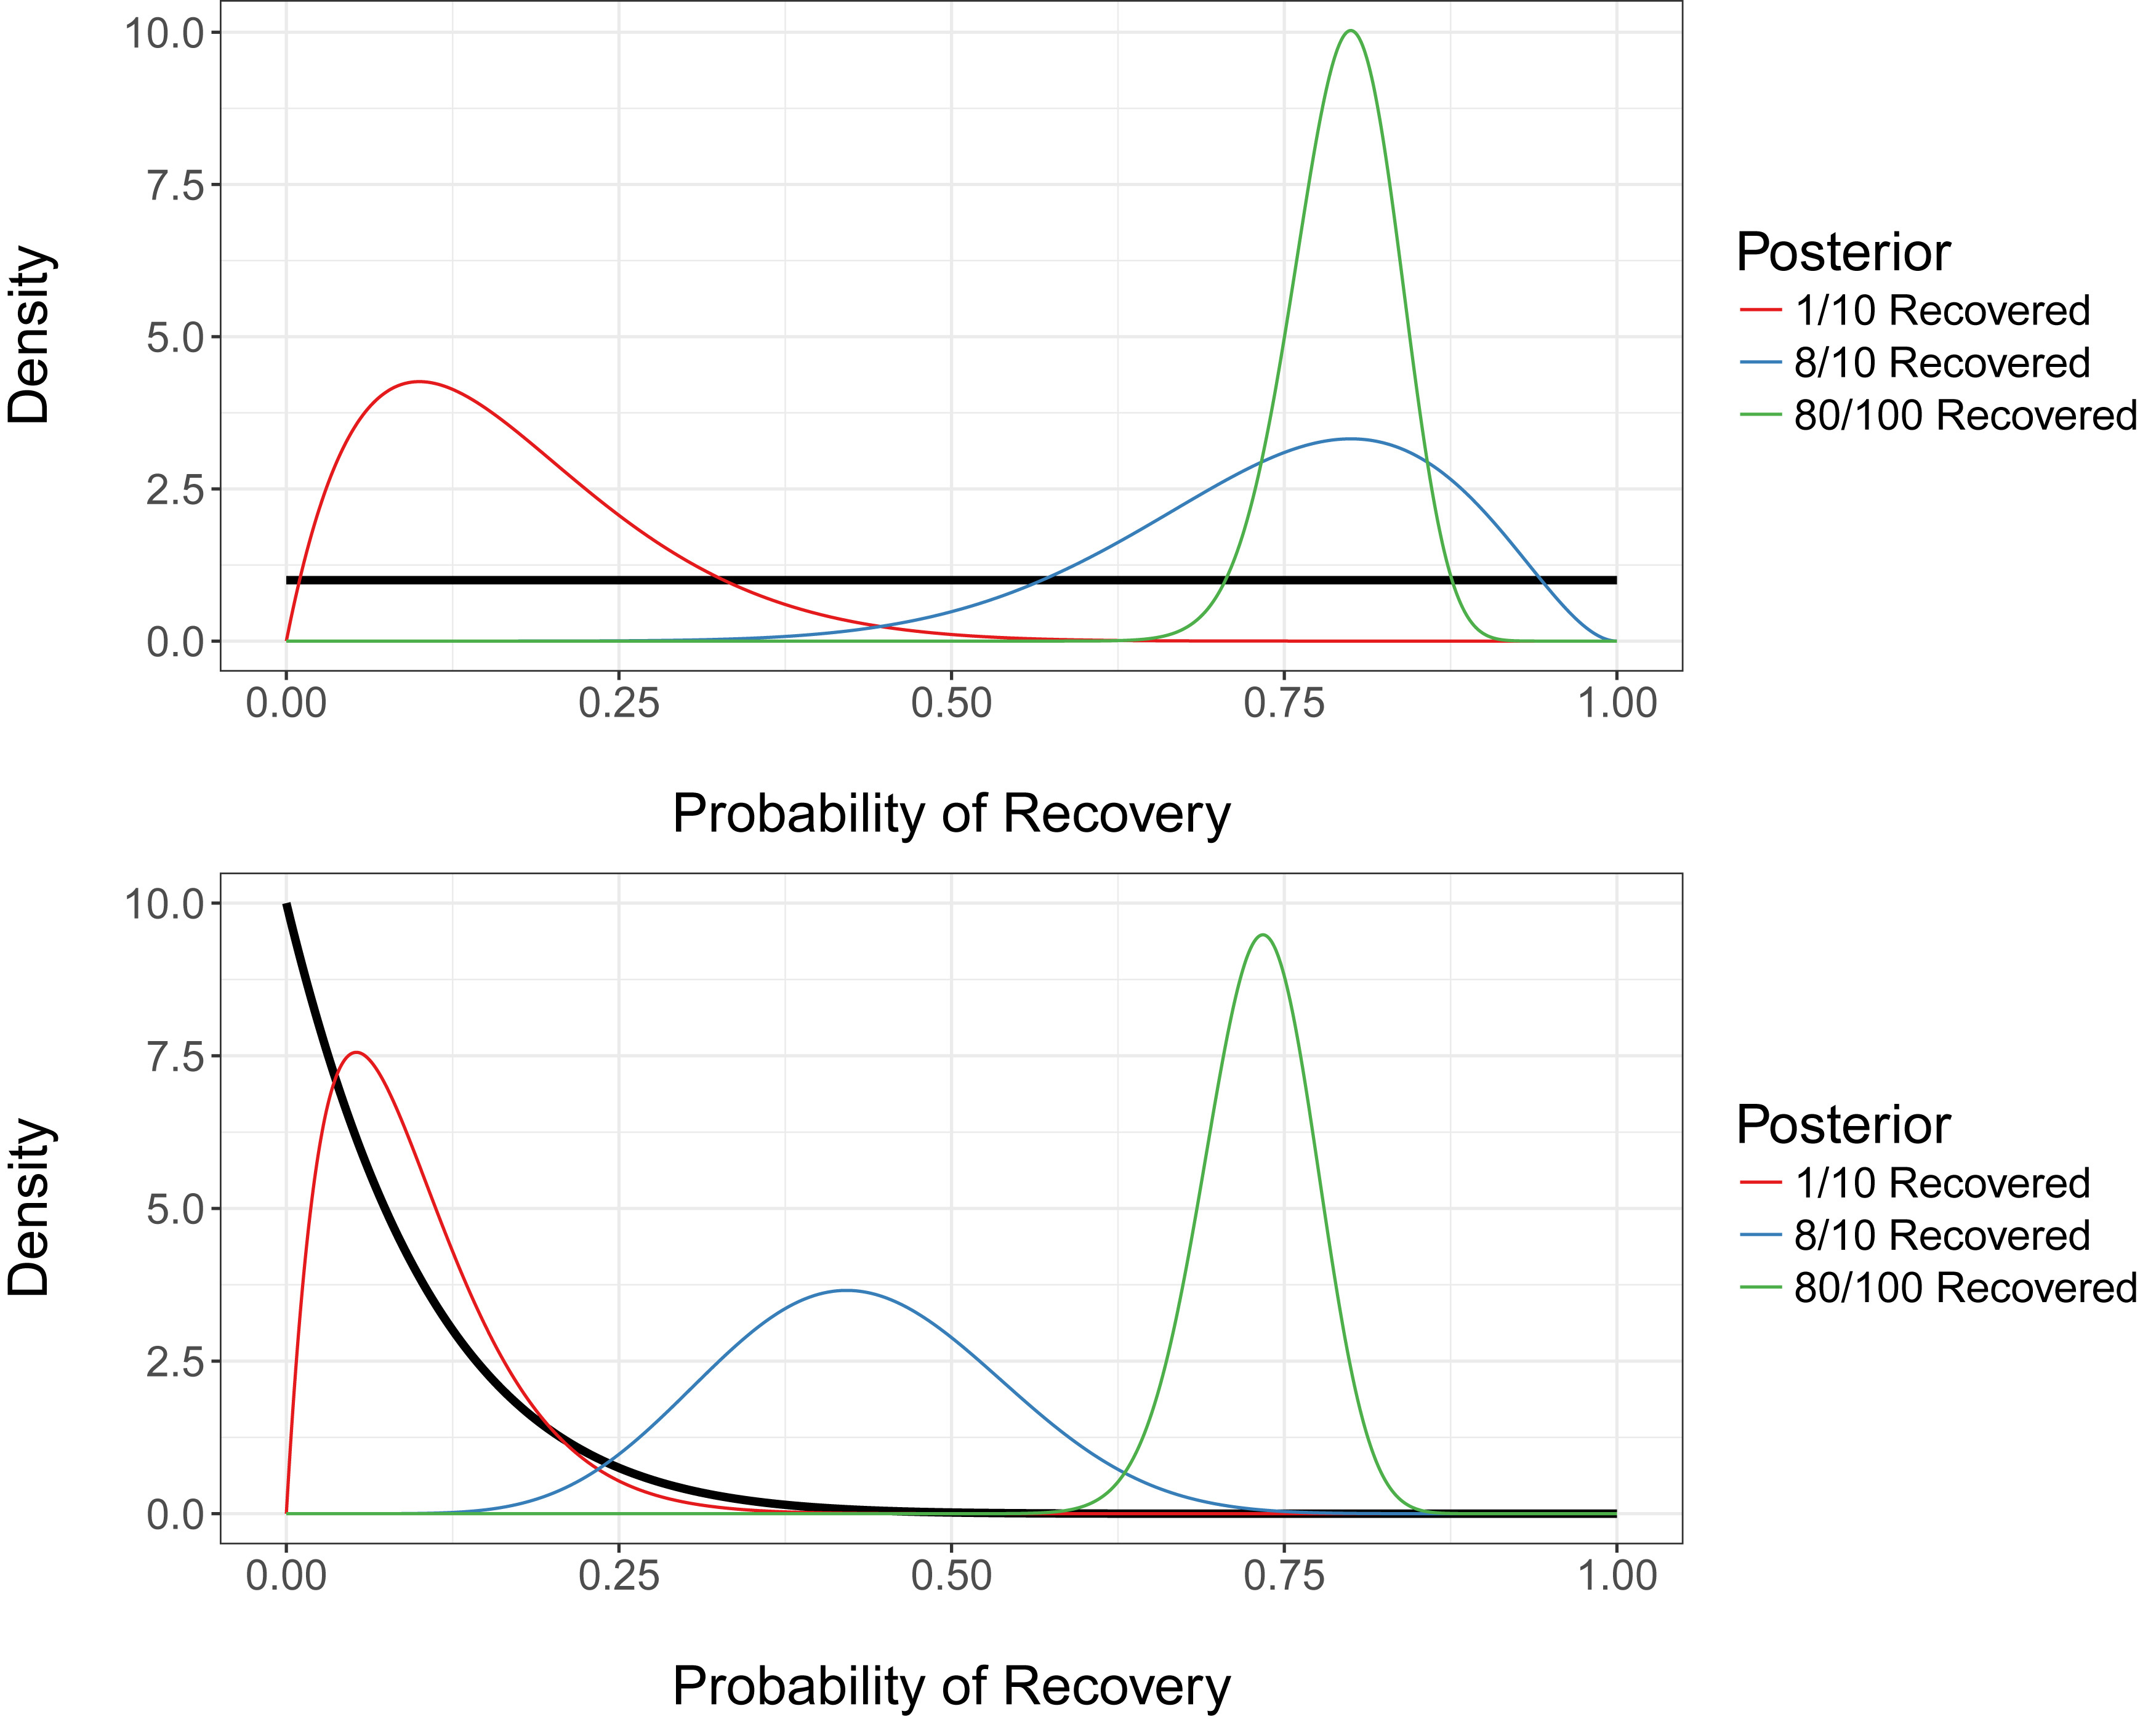
\includegraphics[width=0.5\textwidth]{../imgs/prior-impact.jpg}
  \end{center}
  \caption{Plots demonstrating the impact of different priors and data on posterior distributions. The top figure is for a flat prior distribution and the bottom figure is for an informative prior distribution. Solid black line is the prior distribution, colored lines are the posterior distributions, \cite{clinical}. The flat prior assumes nothing about the recovery percentage beforehand and allows the updated, posterior belief to be fully based on the observed data. The informative prior, on the other hand, assumes that the true recovery percentage is far more likely to be at 0\%, descreasing exponentially for higher recovery values. When little data is available, the posterior distribution is heavily influenced by the prior distribution, but, as more data is collected, the prior distribution has less and less influence on the posterior distribution as the assumptions it makes are being diluted by the data.}
  \label{fig:prior-impact}
\end{figure}
Priors are often a talking point in the validity of experiments using a
Bayesian approach as, while the incorporation of prior knowledge can be a critical
factor in Bayesian models outperforming other frequentist models, especially
when the amount of data is limited \cite{priorgood}; they can also be seen as a
daunting source of subjectivity \cite{clinical}. There are two main
philosophies regarding selecting priors, objective and subjective
Bayesianism \cite{obj-sub}. 

\textbf{Objective Bayesianism} aims to minimise the influence of personal
beliefs on the analysis by using priors that are as non-informative as
possible. Objective priors, often called non-informative or reference priors,
are chosen based on the principle of indifference, which tries to represent a
state of ignorance about the parameters. The goal is to allow the data to have
the most influence on the posterior distribution. This approach is often
favoured when there is limited or non-informative prior knowledge or when
researchers wish to avoid potential bias from subjective beliefs. However, even
with the best intentions in mind, no prior can be truly non-informative, and
objective priors can still carry some level of subjectivity in their selection.

\textbf{Subjective Bayesianism}, on the other hand, embraces the idea that
personal beliefs and prior knowledge should be incorporated into the analysis.
Subjective priors are chosen based on a researcher's knowledge, expertise, and
beliefs about the parameters of interest. This approach allows for integrating
existing information and expert opinions, which can result in
more accurate and informative inferences, especially in cases where data are
limited or noisy. Some argue that subjective priors can introduce bias, as they
rely on the researcher's personal beliefs. However, the opposing argument is that
scientific research is inherently subjective to some degree, and transparency
about the choice of priors, at worst, allows for honest evaluation and discussion
within the research community.
This article by Baldwin and Larson \cite{clinical} explores the viewpoint
that, on the surface, it might seem outright wrong that two otherwise identical
experiments can yield different results simply because different prior beliefs
were defined. Baldwin and Larson show that this argument is mitigated by the
fact that subjectivity is inherent in research, researchers' background
knowledge informs prior choices, all statistical methods involve assumptions
and data likelihood choices often have a more significant impact than priors. They claim
it is justifiable from a scientific standpoint to integrate prior parameter
knowledge into the models. That being said, priors should always be carefully
selected and their impacts transparently communicated.

Both philosophies are worth considering when selecting priors, and while this
paper is grounded more in the objective approach, the subjective approach is
also considered.

\subsubsection{Markov Chain Monte Carlo}

Computing the evidence term, or marginal likelihood, $P(D)$, involves
integrating over all possible values of the parameters, which is often
computationally infeasible \cite{mcmc}. Remember, the posterior distribution is
proportional to the product of the likelihood and the prior, but this
relationship is not absolute due to an elusive normalising constant, the
evidence term, which often complicates the equation. This complexity introduces
the necessity for sampling. Therefore, instead of directly computing the posterior
distribution, which can be a challenging task, it is approximated with the
process of intelligent sampling, avoiding the need to compute the probaility of seeing the data $P(D)$. 

Markov Chain Monte Carlo (MCMC) is the name for a class of algorithms whose
goal is to draw samples from a distribution without needing to know the
specific probability density at any point. From a high level, MCMC achieves
this with a stochastic exploration of the parameter space, guided by the
likelihood function, which reveals regions of higher posterior probability. The
likelihood function answers the question: given this sampled instance of the
parameters, how likely is it that the model generated the observed data?
Areas with higher probability are then explored - or sampled from - more
frequently in the parameter space. The result is a set of samples drawn from a
distribution \textit{proportional} to the posterior distribution. With enough
samples, the posterior can be approximated by the distribution of the samples.
Further reading on MCMC can be found in \cite{mcmc}, as well as alternative
methods for approximating the posterior distribution, such as Variational
Inference \cite{vi}, but deeper understanding of these methods is not required
for this paper.

In this study, the MCMC algorithm employed is the No-U-Turn Sampler (NUTS), an
extension of the Hamiltonian Monte Carlo (HMC) algorithm \cite{nuts}. 
\textbf{Assessing Convergence}\\
As the number of samples increases, the MCMC distribution converges to the
stationary distribution \cite{mcmc}. The stationary distribution is the distribution that 
the MCMC algorithm tries to sample from, i.e. the posterior distribution. 
However, there is no universal threshold for the number of samples required to
reach convergence, so assessing convergence is an essential step in the fitting
process. 

Parameters of the MCMC sampling algorithm defined in this study include:
\begin{itemize}
  \item \textbf{Draws} - The number of samples to draw from the posterior
  \item \textbf{Tune} - The number of samples to discard as burn-in. Burn-in refers to the 
  number of samples to discard before the samples are considered to be from the stationary 
  distribution \cite{mcmc-convergence}.
  \item \textbf{Chains} - The number of chains. Chains are independent runs of
    the MCMC algorithms started from different values to check that a
    reliable posterior estimate is obtained \cite{mcmc-convergence}.
  \item \textbf{Target\_accept} - The desired acceptance rate for proposed moves during the sampling process.
\end{itemize}
Convergence diagnostics defined in this paper include include:
\begin{itemize}
  \item \textbf{mcse\_mean} - Monte Carlo Standard Error of the Mean
  \item \textbf{mcse\_std} - Monte Carlo Standard Error of the Standard Deviation
  \item \textbf{ess\_bulk} - Effective Sample Size for the Bulk
  \item \textbf{ess\_tail} - Effective Sample Size for the Tail
  \item \textbf{r\_hat} - Gelman-Rubin Diagnostic
\end{itemize}
The Monte Carlo Standard Error (MCSE) is a measure that helps in understanding
the precision of the MCMC estimates. It quantifies the uncertainty in
estimates due to the simulation process involved in MCMC. The lower the
MCSE, the closer we can expect our MCMC estimate to be to the actual value.
The MCSE comprises two components: the mean MCSE, which measures the
uncertainty in estimating the mean of the posterior distribution, and the
standard deviation MCSE, which assesses the precision in estimating the
standard deviation of the posterior distribution.

The value of the Gelman-Rubin diagnostic (R-Hat) provides evidence that the
multiple chains converged to the same posterior distribution by measuring the
between-chain and within-chain variance ratio. Values close to 1 indicate
convergence and values greater than 1.1 are considered to demonstrate
non-convergence \cite{statrethinking}.

Effective sample size (ESS) is a measure of the number of independent samples
that would be required to achieve the same precision as the MCMC samples. The
ESS for the bulk is the ESS for the samples excluding the first 50\% of the
samples, and the ESS for the tail is the ESS for the samples excluding the
first 10\% \cite{statrethinking}. Ideally, the ESS should be close to the
number of samples drawn. 
\subsubsection{Trace Plots}
Trace plots are a valuable tool for visualising the MCMC sampling process. They 
show the value of each parameter throughout the sampling process, 
allowing for manual convergence assessment and identification of potential problems with
the sampling process.
A trace plot is a line graph where the x-axis represents the iteration, and the
y-axis shows the sampled parameter value. Trace plots, such as those generated
in \texttt{Arviz} with \texttt{plot\_trace()}, should exhibit two key
characteristics: stationarity and good mixing \cite{statrethinking}.
Stationarity implies that the samples remain within the posterior distribution
and accurately represent it \cite{puppies}. In other words, the trace plot
should not deviate outside the posterior distribution but maintain its position
within the same parameter space throughout iterations and chains. Good mixing
signifies that consecutive samples within a chain should not be correlated.
Instead, the trace plot should oscillate within the posterior, moving both
upwards and downwards, indicating that the chain is collecting samples from all
areas of the posterior or thoroughly exploring the posterior distribution. 
\begin{figure}
  \begin{center}
    \includegraphics[width=0.7\textwidth]{../../eval/SimpleTemp/90/trace.png}
  \end{center}
  \caption{\textbf{Example Trace Plot} (for model $M_1{-}0{-}90$) displaying the Markov chain Monte Carlo (MCMC) sampling for the beta, sigma, temperature, and weekday parameters. Each subplot represents the trace of one parameter, providing an insight into the convergence and mixing of the chains. The plots reveal the posterior distribution of the parameters, essential for understanding the uncertainty and variability in the model's estimates.}
  \label{fig:trace-plot}
\end{figure}
\subsubsection{Autocorrelation} 
Autocorrelation is a statistical measure that quantifies the similarity between
observations of a series conditioned on a specific time lag, where a lag is a
fixed distance between time steps \cite{time-series2}. The concept has been mentioned in the
context of MCMC sampling but is arguably more traditionally associated with
time-dependent data, such as the present case study. While the concept remains
the same, it is vital to understand the implications of autocorrelation in both
contexts.

\textbf{Autocorrelation in MCMC sampling} refers to the dependence between
samples in the MCMC chain. Since MCMC methods generate samples sequentially,
consecutive samples can be correlated. High autocorrelation
between samples indicates that the MCMC chain is moving slowly through the
parameter space and not exploring the posterior distribution efficiently \cite{mcmc}.
Autocorrelation in MCMC samples is undesirable, as it reduces the effective
sample size, leading to less precise estimates of the posterior
mean, variance, or other quantities of interest \cite{mcmc}. To assess the autocorrelation
in MCMC samples, we calculate the autocorrelation at different lag times within
the chain, where a lag refers to the difference in positions between two
samples. If the autocorrelation is high, it suggests that the MCMC sampling
process is inefficient. The chain might need to be run for more iterations, use
a different MCMC algorithm, or adjust the tuning parameters to improve the
sampling efficiency \cite{andrieu2003introduction}.

\textbf{Autocorrelation in time series data} measures the degree of similarity
between a variable's current value and its past values a certain number of
"lags" away. Here, a lag refers to the time difference between two
observations. If a time series has strong autocorrelation, it means that the
values of the series at different time points are highly dependent on each
other \cite{time-series1}. This information is helpful for time series forecasting, as it helps to
identify patterns and trends in the data that can be exploited to make more
accurate predictions. For instance, if a time series exhibits high positive
autocorrelation at a specific time lag, it suggests that the values at that
time lag are similar to the current values \cite{time-series2}. Conversely, if the time series
exhibits high negative autocorrelation, it implies that the values at that time
lag are dissimilar to the current values \cite{time-series2}. Knowing the autocorrelation structure
of a time series can be crucial for selecting appropriate forecasting models,
such as autoregressive (AR) models, which use past values as predictors for
future values.

\subsection{Bayesian Model Comparison \& Evaluation}
\subsubsection{Metrics}
\label{subsec:metrics}
Bayesian statistics includes its model comparison philosophy, which will be applied to compare and select the best of the various models
later in the study. The Bayesian approach to model comparison aims to identify
the model that achieves the best trade-off between goodness of fit and model
complexity in order to provide the most accurate and informative explanation
of the observed data.

In order to evaluate the predictive capability of the various models and make
comparisons between them, it is essential to define specific performance
metrics. These metrics provide quantitative measures of the accuracy and
precision of the model's predictions.

\begin{itemize}
\item \textbf{Mean Absolute Error (MAE)}: This metric computes the average absolute difference
between the predicted and actual values, providing a straightforward measure of
the model's accuracy. A lower MAE value indicates better performance, showing that the model's predictions are closer to the actual values.

\item \textbf{Mean Squared Error (MSE)}: The MSE calculates the average squared difference
between the predicted and actual values. By squaring the errors, this metric
gives more weight to larger errors. This means that a model with a lower MSE is
accurate and consistent in its predictions.

\item \textbf{Root Mean Squared Error (RMSE)}: The RMSE is the square root of the MSE. It is
in the same units as the target variable, making it more interpretable than the
MSE. Like the MSE, a lower RMSE indicates better performance.

\item \textbf{Mean Absolute Deviation (MAD)}: The MAD measures the dispersion of the errors
around their mean. A lower MAD indicates that the errors are tightly clustered
around their mean, suggesting that the model is reliable and stable.

\item \textbf{Earth Mover's Distance (EMD)}: Also known as the Wasserstein
  distance, EMD measures the distance between two probability
  distributions. Unlike the other metrics, EMD does not simply compare the
  predicted and true values but rather the entire distribution of these
  values. This metric is particularly useful in the context of Bayesian models,
  where predictions are distributions rather than single-point estimates. 

\item \textbf{Logarithmic Probability Density (LPD)}: A measure of the model's
ability to accurately predict the probability distribution of the target
variable. A higher LPD indicates that the predicted distribution more closely
matches the actual distribution, implying better model performance.
\end{itemize}

Richard McElreath motivates and explains techniques for Bayesian model
comparison in great detail in his book on Bayesian Data Analysis
\cite{statrethinking}. For this paper, complete knowledge of the inner workings
of the techniques is not required; however, it helps to understand the intuition
behind the techniques foundational to the Bayesian approach to model
comparison.

\begin{itemize}
  \item \textbf{Bayes Factor} - A measure of the relative evidence of one model
    over another, calculated by taking the ratio of the marginal likelihoods of
    two models, asking: Which model is more likely to have generated the
    observed data?
  \item \textbf{WAIC} - Widely Applicable Information Criterion, a measure of
    out-of-sample predictive accuracy, quantifying the trade-off between
    goodness  of fit and model complexity.
  \item \textbf{LOOCV} - Leave-One-Out Cross-Validation, a measure of
    out-of-sample predictive accuracy, iteratively assessing model fit on
    $(len(Data) - 1)$ folds of data.
\end{itemize}

A Region of Practical Equivalence (ROPE) is also used in this study. ROPE is a
Bayesian approach for hypothesis testing, often used to ascertain if a
parameter value can be considered practically equivalent to a null value,
usually zero \cite{puppies}. The concept of ROPE is born from the recognition
that in real-world scenarios, it is often more practical to accept a small
range of values as equivalent to zero rather than insisting on exact equality.
This range of values is what we define as the Region Of Practical Equivalence.
In this study, it is used to determine the significance of a model parameter;
if the ROPE contains falls within the 95\% Highest Density Interval of a
parameter's posterior, then the parameter is considered insignificant for all
practical purposes \cite{puppies}.
The Highest Density Interval (HDI) is another crucial concept in Bayesian
statistics. It represents the range of values that contain a specified
proportion, typically 95\%, of the posterior distribution. The HDI provides a
credible interval for parameter estimates, offering an intuitive understanding
of uncertainty in Bayesian analysis \cite{statrethinking}.

\subsubsection{Pearson Correlation Coefficient}

The Pearson Correlation Coefficient (PCC) is a measure of the linear
relationship between two continuous variables. It ranges from -1 to 1, where -1
indicates a perfect negative linear relationship, 1 signifies a perfect
positive linear relationship, and 0 suggests no linear relationship. The PCC is
sensitive to outliers and assumes that the variables are normally distributed.
Therefore, it may not accurately capture relationships that are not linear or
data sets that do not follow a normal distribution.

\subsubsection{Kendall's Tau}

Kendall's Tau is a non-parametric measure of correlation that evaluates the strength and direction of association between two ranked variables. It can be used for continuous, ordinal, and discrete variables. Unlike PCC, Kendall's Tau is not influenced by outliers and does not require the data to follow a specific distribution. Kendall's Tau values also range from -1 to 1, where -1 indicates a perfect inverse relationship, 1 signifies a perfect direct relationship, and 0 suggests no relationship. It is particularly effective in identifying rank correlations, where it's not the actual values but the order of the data that matters.

\subsubsection{Bayes Factor}

Bayes' factor represents the relative evidence favouring model $M_1$ over
model $M_2$. If $BF_{1,2}>1$, then the data provide more evidence for $M_1$
than $M_2$, while if $BF_{1,2}<1$, the data provide more evidence for $M_2$
than $M_1$ \cite{statrethinking}. 
Measuring the log-likelihood of the true test data and the model's predictive
distribution for the test observations is another useful approach to assess the
model's predictive performance. This is also known as the log predictive
density (LPD), which is used to quantify the model's ability to predict new,
unseen data. The log-likelihood is used instead of the likelihood for each
point for the numerical stability, simplicity, and interpretability of logging
the values.
Bayes' factor can be calculated by subtracting the LPD since; we assume that
the models are equally likely a priori; the Bayes' factor is the posterior odds
of the models. 
Bayes' Factor can be derived from Bayes' theorem and calculates the posterior
odds of the models, assuming that the models are equally likely a priori.
First, we start with Bayes' theorem:
\begin{equation}
p(\theta|D,M) = \frac{p(D|\theta,M)p(\theta|M)}{p(D|M)}
\end{equation}
The marginal likelihood or evidence, $p(D|M)$, is given by integrating the numerator over all possible values of $\theta$:
\begin{equation}
p(D|M) = \int p(D|\theta,M)p(\theta|M) d\theta
\end{equation}
This marginal likelihood $p(D|M)$ is what we are interested in for calculating the Bayes' Factor.
The Bayes' Factor for comparing models $M_1$ and $M_2$ is defined as the ratio of their marginal likelihoods:
\begin{equation}
BF_{1,2} = \frac{p(D|M_1)}{p(D|M_2)}
\end{equation}
Beyond model selection, Bayes' Factor provides a subtle balance
between model fit and complexity. The model fit is assessed by the
likelihood term of the Bayes' Factor calculation, $p(y|\theta_{i},M_{i})$. A
model that fits the data well produces a high likelihood value, which increases
the Bayes' Factor in favour of that model. On the other hand, model complexity
is addressed by the prior probability of the model parameters,
$p(\theta_{i}|M_{i})$. For example a complex model with many parameters might provide a
better fit to the data, but each additional parameter also needs additional
prior assumptions. Suppose these assumptions are not well-supported by the data. In that case the
prior probability of the parameters can become very low, thereby reducing the
overall marginal likelihood of a more complex model. The Bayes Factor considers
both aspects by integrating over all possible parameter values, providing a balance
between fit and complexity.
\subsubsection{Log Pointwise Predictive Density}
LPD is the logarithm of the probability of the data given the model. With
model $M$ and a dataset $D$, the LPD is calculated as follows:
\begin{equation}
  \begin{split}
    LPD &= \log p(D|M) \\
    LPD &= \sum_{i} \log p(y_i|\theta, M)
  \end{split}
\end{equation}
Where $y$ are the observations in the dataset, and $\theta$ are the parameters
of the model. The crucial part: under certain assumptions (like the
models being equally likely a priori), the difference in LPD is equivalent to
the log of the Bayes' Factor:
\begin{equation}
  \begin{split}
    BF_{1,2} &= \frac{p(D|M_1)}{p(D|M_2)} \\
    \log BF_{1,2} &= \log \frac{p(D|M_1)}{p(D|M_2)} \\
    \log BF_{1,2} &= \log p(D|M_1) - \log p(D|M_2) \\
    \log BF_{1,2} &= LPD_1 - LPD_2
  \end{split}
\end{equation}
When comparing two models using LPD, subtracting the LPD of the two models to
get the log of the Bayes' Factor can then be used as a proxy for the Bayes Factor
due to the monotonicity of the log function: $\log(x) > \log(y) \iff x > y$.
The only practical difference is that the threshold for equal evidence changes from  
$BF_{1,2} = 1$ to $\log BF_{1,2} = 0$.

\subsection{Data Volume and Performance}
The second research question asks: What is the optimal data volume for accurate
revenue prediction? This intuition is based on questioning the common
assumption that the more data is available, the more accurate the model will
be. In the real world, there is no guarantee that the complicated underlying
revenue-generating process will remain constant over time; therefore, there
exists the possibility that incorporating data from the distant past will not
only not lead to better predictive power but, by introducing more noise, may
lead to worse predictions. This is an area that has been researched but lacks
a clear consensus. 
The importance of considering data quality and recency when incorporating
historical data in econometric models has been highlighted
\cite{big-data-hal-varian}. Hal Varian suggests that using too much historical
data or data that is not directly relevant to the problem at hand can sometimes
introduce noise and lead to worse predictions. However, when this notion is
explored in another article \cite{data-volume-weather}, the authors find that
more data is categorically beneficial in improving the accuracy of a trained
model. To this end, this study aims to explore the relationship between data
volume and predictive power in the context of Bayesian revenue modelling and
forecasting.
